\section {Contributions from the study}\label{contributions}
The emission factors for combustion engines, as used in the national emission inventories, are based on measured emissions from standardised test runs \cite{Andre2004}, and are used for a bottom up estimate of the total national emissions, by estimating the number of kilometres the total national fleet have driven \cite{nielsen2014}. This estimate is compared to an estimated emission calculated from the amount of gasoline and diesel sold nationally, and the difference between these two estimates leads to a correction factor for the total national emission.

\subsection{Simple emission model}

A simple model for estimating the emissions from single trips has been developed. The trips are divided into sections by the transportation mode detection algorithm. For each transportation mode an emission factor is calculated and multiplied with the length of the section. The total emission for a trip is calculated by accumulating the emissions from the sections. The emission factors for cars, trucks, busses and trains are derived from the reporting of the national emission inventories to UNFCC under the Kyoto Protocol. 

When using smartphones as mobile sensing devices, a number of different sensors can be used. In the following the builtin accelerometer and the global positioning sensor are considered. The accelerometer sensor, delivers a timestamped accelerometer measurement, consisting of a reading of the 3 axis accelerometer. The accelerometer is a very low power device and can thus be sampled more frequently ( around 200 Hz ) \cite{Kjaergaard2009}.

The GPS measurements consists of longitude, latitude, altitude, speed, bearing, number of satellites visible, accuracy and a timestamp of the measurement. The GPS sensor contains a radio receiver, and complex logic to decode the radio signals from multiple satellites and calculate a position from the data, thus it uses more electric power. To reduce the power drain on the smartphone battery, the GPS can be turned off between readings of the position. 



When calculating the distance travelled between two GPS measurements a Haversine function is used. This function takes the curvature of the earth into account, and therefore gives a more precise value for the distance. The resolution of the test data, does not warrant the use of the Haversine approach, since it is sampled every second, but was chosen in anticipation on more crudely sampled GPS data, due to power conservation considerations.
\begin{figure}[!ht]
\begin{center}
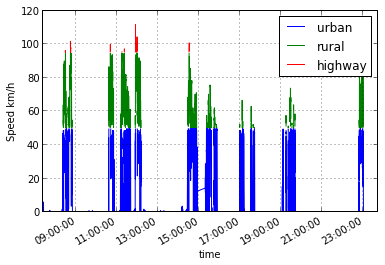
\includegraphics{speed_division.png}
\caption{{\bf Dividing driving into urban, rural and highway}}
\label{speed_division}
\end{center}
\end{figure}

The emissions are estimated for 3 different driving patterns: Urban, with many stops and low speed. Road driving, with few stops and moderate speeds, and lastly highway, with no stops and high speed. These three modes of road traffic can be distinguished by analysing GPS.  In figure \ref{speed_division} an example of a speed curve for a series of trips and how the different driving types the trips are dived into. The distance travelled for each road type can be found by adding the distance between sampling points for points in each driving type. These distances are multiplied with the emission factors from the Tier 3 methodology.

\begin{figure}[!ht]
\begin{center}
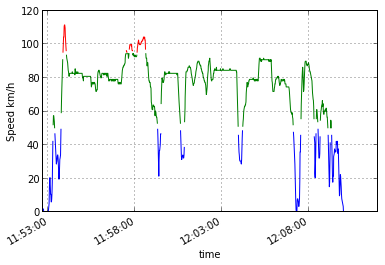
\includegraphics{speed_division_zoom.png}
\caption{{\bf A closer look on figure \ref{speed_division}}}
\label{speed_division_zoom}
\end{center}
\end{figure}

In figure \ref{speed_division_zoom} a closer look on figure \ref{speed_division} is shown. From the figure it can be seen that the division with fixed speed limits delivers a quite crude division and gaps where the speed changes a cross a boundary between road types. 

\subsection{Enhanced emission model}

\begin{figure}[!ht]
\begin{center}
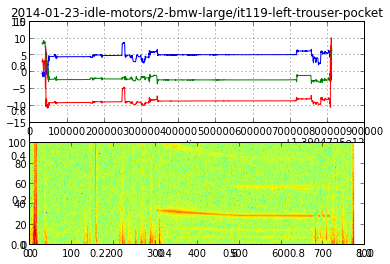
\includegraphics{idle_BMW.png}
\caption{{\bf Engine revolutions. The top figure shows the three accelerometer signals. The bottom figure is the spectrogram of the size of the acceleration vector}}
\label{idle_bmw}
\end{center}
\end{figure}

To create a more accurate estimate of the emission for a single trip by car, a more complex model is proposed. From the sensed data it is possible to get information on the speed of the car at various points of the trip, and the number of stops and starts. This information can be used to further segment the trips into idle, accelerating, cruising and braking; each of these segments would have a different emission profile. 

The data sensed from the smartphone can also be used to determine if the engine in the car is cold, if for instance it is the start of the trip. When the engine is cold the combustion and the catalytic converter are less effective,and thus more emissions of Carbon Monoxide and Volatile Organic Compounds will be higher and the emission inventory should reflect that. The determination of the impact of cold starts, demands a quite complex models, taking into account the outside temperature, models for engine warm up \cite{Ntziachristos2012}. 


\subsection{Determine Idle engine revolutions}
By analysing the frequency spectrum of the accelerometer data, information on the engine revolutions can be retrieved \cite{markus2014}. By employing spectrograms (shows the time evolution of spectral features)  changes in engine speed can be visualised. An example (see figure  \ref{idle_henrik}) is the the idle speed of a cold motor, where the ECU (Electronic Control Unit) of the vehicle, measures the temperature of the motor and as long as the motor is too cold, sets the idle speed at a higher value. The lowering of the idle speed as the engine grows warmer, is clearly visible in the spectrogram.
The spectrogram is calculated by calculating the size of the accelerometer vector, i.e.:

\begin{center}
$a = \sqrt{x^2+y^2+z^2}$
\end{center}

By assuming that the smartphone is kept still or only moved slowly, the gravity can be considered constant. The gravity will be present as a signal with frequency equal to zero, which can easily be removed, as it is the zero'th element in the array returned by the Fast Fourier Transform (FFT). So even though the gravity is a very large signal and the signal stemming from vibrations in the engine are quite faint, it is possible to filter the gravity out \cite{Hemminki2013}.

\begin{figure}[!ht]
\begin{center}
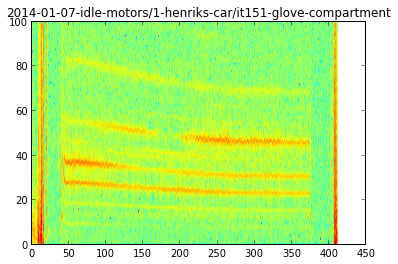
\includegraphics{idle_henrik.png}
\caption{{\bf figure showing rotational speed of an cold engine. As the engine heats up the the engine speed lowers. The yellow and red colours indicates larger powers in that frequency range.}}
\label{idle_henrik}
\end{center}
\end{figure}

The spectrogram shows the time evolution of the frequency spectrum of a signal, so the y-axis shows the frequencies, and the x-axis shows the time. The size of individual frequencies is shown by using different colours. A constant frequency will result in a horizontal line in the spectrogram, and slowly varying frequencies will result in curves in the spectrogram. The usefulness of the spectrogram is to show signals with few  frequencies that change slowly, and not to ascertain the exact size of individual frequencies. The spectrogram can therefore be said to be a qualitative display technique.

An example of a spectrogram of a car in idle mode is shown in figure \ref{idle_bmw}. The slowly decreasing red line coincides, timing wise, with the engine starting. As the engine warms up the engine speed can be seen to slow. The actual frequency of the red line indicates that it probably is a harmonic of the basic frequency.
  
During driving, the vibrations from of the moving car, that is the vibrations of from the tires moving over the road and vibrations from the transmission system, drowns the signal of the engine rotational speed.

Another effect that contributes to the loss of a clear signal for the rotational speed of the engine is due to the low sampling frequency of the accelerometer. The sampling frequency of the accelerometer i approximately 200 Hz. This means that the data from the accelerometer only can represent signals with frequency below 100 Hz, due to the Nyquist criteria. This maximum frequency of 100 Hz corresponds to a engine speed of 6000 rpm. Thus the sampling frequency only allows for accurately representation of frequencies below 6000 rpm, and if higher vibrational frequencies exists these frequencies will be folded back into the spectrum from 0 to 6000 rpm, a process called aliasing \cite{lyons2010understanding}. Since combustion engines often employ more than one cylinder, and since the process of combustion takes place as a violent process in the cylinder, it is reasonable to expect harmonics of the engine speed to be created. When the engine is in idle mode a rotation of 900 - 1000 rpm (15 - 16,7 Hz) is normal and the sampling of the accelerometer will allow the correctly represent up to the sixth harmonic, but when the vehicle is driving engine rotation speed between  
2000 - 3000 rpm would be appropriate, thus only allowing to represent third or only second harmonics. Any higher order harmonics will be aliased back into the spectrum and contribute to the noisy picture. 

As a result of vibrational noise from the moving vehicle and aliasing of engine vibration (and aliasing of the vibrational noise for that matter) the signal from the engine rotation is lost in the noise. In signal analysis, the way to prevent aliasing is to apply a low pass filter to remove or dampen frequencies above half the Nyquist frequency. But in our application it is not possible to ensure that the smartphone containing the accelerometer is adequately shielded from high frequency vibrations.

One method used for exploration of the data from the accelerometer, was to convert the signal into an audio file and listen to different types of transportation. By playing the audio file at a higher sampling frequency than the accelerometer sampling frequency, low frequency tones are more easily recognised as their frequency will be multiplied by the increase in sampling frequency. The time used for listening is shortened with the same factor. A factor of 5 was used to examining the data. Since the human hearing is quite adept in separating single frequencies, it is a good way to quickly ascertain if patterns are available in the data.

From the datasets used in this study, it we conclude that it is possible to detect idle mode, for vehicle with combustion engines. Other types of vehicles, like electric vehicles or vehicles that stop their engine when the vehicle stops, would not need a idle mode detection.

\subsection{Determine acceleration and turning}
I order to distinguish between the the four modes of driving (idling, accelerating, cruising, decelerating), which have different emission characteristics, we can use the accelerometer data to determine the the acceleration patterns in the horizontal plane.

The data from the accelerometer is 3 values for each measurement, which are the 3 axis from the accelerometer. The direction of movement of the phone can be determined by analysing these 3 signals. First the direction of gravity is determined . Since it is possible for the phone to be moved freely in all directions and/or flipped with the movement of the person wearing the phone, the gravity detection needs to be dynamic \cite{Hemminki2013}. When the direction of gravity has been determined, it is possible to detect acceleration in the horizontal plane. This allows us to consider distinguishing turning from linear acceleration, which is important because a linear acceleration will have a different emission factor than turning.

\subsection{Combine turning information with GPS }

By combining the turning information, with GPS localisation and map data, the accuracy of the positioning of the car can be improved. Improving the positioning accuracy is important for improving the accuracy of the calculation of trip length and segment of trips length.

The more accurate trip emission estimate would be of interest for green accounting purposes.

The combination of turning information with GPS location will also improve the detection of acceleration and deceleration driving modes, and thus improve the emission estimate.


To validate and compare the models the exact emissions can be measure by inserting a sensor into the exhaust pipe of the vehicle under test. By doing test runs in different kinds of traffic, and with different vehicles the results of the sensor can be compared with the results of the models see section \ref{futurework}.

By combining the GPS data and the accelerometer data, we can detect cruising mode, and maybe acceleration/deceleration.